\section{Concept}
To be able to meet the requirements of our interactive floorplan, the events from the gates need to be logged and displayed in real-time. For this to work, there are multiple components involved. A general overview about the architecture can be seen in figure 3.

\begin{figure}[!hb]
	\centering
	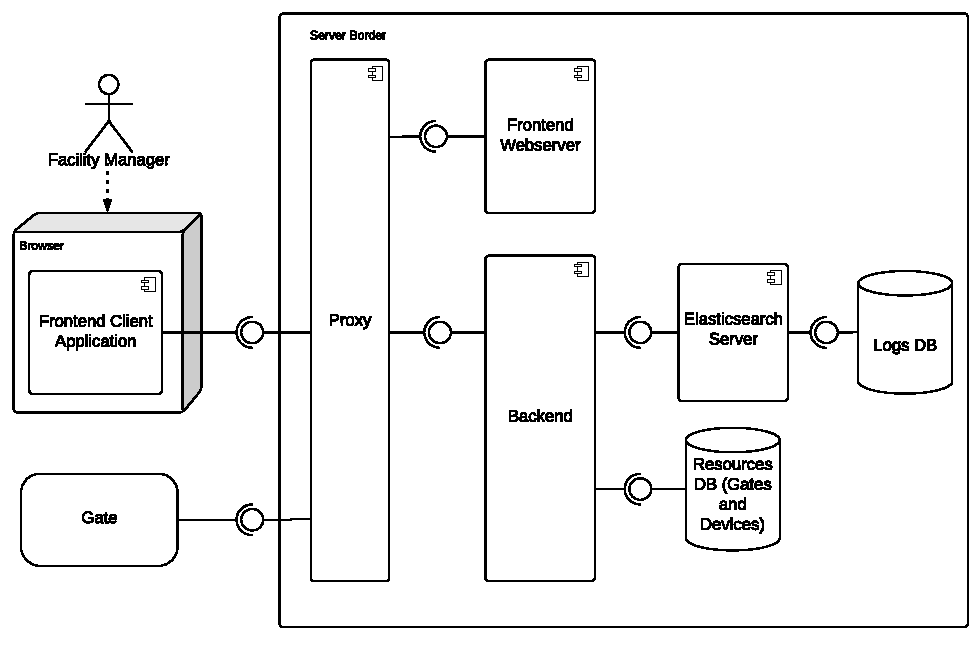
\includegraphics[width=1\linewidth]{images/Komponentendiagramm}
	\caption{Component diagram}
	\label{fig:Komponentendiagramm}
\end{figure}

\subsection{Gates}
\label{Gates}

The gates take care of capturing different informations once a person tries to access through a gate. They gather information about the device that communicates with them, if they granted or denied the access and if the person tries to enter or exit through the gate. In case of an alarm they need to store other useful information about that incident.

The gate then is responsible of sending this information to our system via an API\footnote{Application Programming Interface}.


\subsection{Backend}
\label{Backend}

The backend offers interfaces for the gates and also the frontend. For the gates it provides an interface which allows the gates to send events to, which then will be persisted as logs.
For the frontend it provides routes for retrieving the logs and also analytical results based on these.

Once a gate transmits data through the available interface, the backend emits a notification that an event occured together with the event data. 


\subsection{Frontend}
\label{Frontend}

The frontend presents the interactive floorplan to the facility management with clickable markers for each gate.
It features the adding and deleting of markers and the possibility to link them to a gate.
A click on a specific marker shows useful informations about the gate, such as the minimal entry and minimal exit trust level required for this gate.

For the possibility of displaying data in real-time, it listens for the gate event notification sent from the backend. When a notification is emitted the frontend the event data gets visualized to the user. This also triggers a recolorization of the room that is connected to the gate where the event occured, thereby showing the up-to-date occupancy of that room.

\subsection{Logging Server}
\label{Logging Server}

The logging server takes care of storing the events in a log database. It offers endpoints for creating event logs and also for searching through the logss. This allows to calculate the number of people in a room for example.

\clearpage



